\subsection{Атомный фактор рассеяния}
Рентгеновское излучение, взаимодействуя с электронами атомов вещества рассеивается.
Величина такого рассеяния зависит от количества электронов в атоме. Тяжелые металлы,
 например свинец, Pb (Z = 82), рассеивают рентгеновское излучение сильнее легких,
 таких как Ni (Z = 28) или  Co (Z = 27), а такие атомы, как He или H – прозрачны
 для рентгеновского излучения. Величина, которая характеризует о том, как сильно
 рассеивает атом, называется атомным фактором рассеяния f.
На рисунке ~\ref{ris:atom_factor} представлена диаграмма направленности атомного
фактора лантана в зависимости от угла, максимальная величина наблюдается в случае
 рассеяния вперед и рассеяния назад.

\begin{figure}[h]
  \centering
  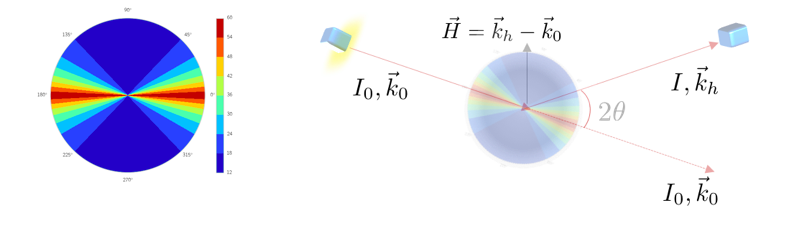
\includegraphics[width=0.9\textwidth]{images/atom_factor.png}
  \caption{ (Слева) фактор рассеяния для атома лантана (La, N = 57), (справа)
  схема расположения векторов для падающей и рассеянной волн}
  \label{ris:atom_factor}
\end{figure}

Приближенное выражение для расчета атомного фактора рассеяния
представляется \cite{International_Tables} в виде выражения:

\begin{equation}
  f_0 = \sum_{i=1}^{4} \cdot a_i e^{ -b_i (\frac{sin \vartheta_B}{\lambda})^2} + C
 \end{equation}
где $a_i$, $b_i$ и $c$ - коэффициенты Кромер-Манна для бездисперсионного канала рассеяния атомами решетки,
ограничением является $0<\frac{sin\vartheta}{\lambda}<2.0 \angstrom ^{-1}$.
 Характерная зависимость структурного фактора от угла рассеяния и длины волны
для атомов входящих в состав кристалла LGT (La, Ga, Ta, O) представлена на рисунке ~\ref{ris:atom_factor_GaLaTa}.

\begin{figure}[h]
  \centering
  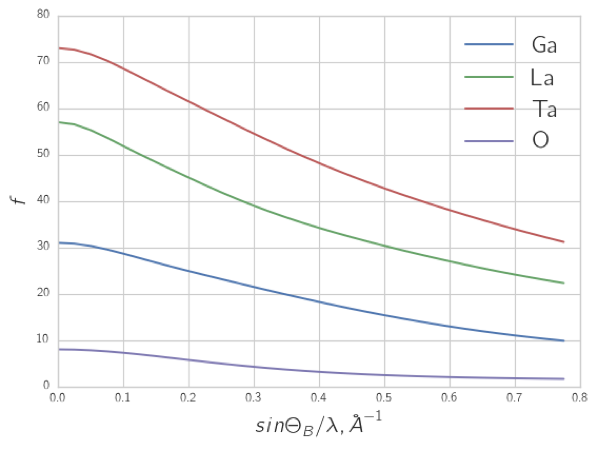
\includegraphics[width=0.9\textwidth]{images/atom_factor_GaLaTa.png}
  \caption{ Атомный фактор рассеяния для атомов: галлия (Ga), лантана (La), тантала (Ta) и  кислорода (O)}
  \label{ris:atom_factor_GaLaTa}
\end{figure}

В общем случае атомный фактор рассеяния является комплексной величиной,
но мнимая часть выражения становится значимой только вблизи края собственного
 поглощения, когда энергия кванта близка к резонансной энергии атома.

 \begin{equation}
   f = f_0 + f^{'} + i f^{''}
  \end{equation}

$f_0$ - атомный фактор рассеяния, независящий от энергии падающего излучения,
$f^{'}$,$f^{''}$ - действительная и мнимая части дисперсионной поправки \cite{f0f1f12},
 обусловленные преломлением и поглощением

 
